\chapter{Modellbildung}\label{chapter: Modellbildung}
\thispagestyle{empty}
Dieses Kapitel stellt dar, wie die verwendeten technischen Anlagen zur Gewinnung von Betriebskennlinien modelliert worden sind. Im ersten Abschnitt wird die verwendete Simulationssoftware \acf{TESPy} vorgestellt. Daran anschließend wird für jede Technologie gezeigt, wie diese in \ac{TESPy} modelliert wurde und welche Daten bzw. Kennlinien konkret aus der Simulation gewonnen werden konnten - alle Modelle können dem beigefügten Datenträger entnommen werden. Außerdem wird gezeigt wie gewonnene Kennlinien für die spätere Optimierung linearisiert worden sind. 

\section{Simulationssoftware - TESPy}\label{section: TESPy}
\ac{TESPy} ist ein Python-Paket, welches zur Simulation thermodynamischer Kreisprozesse genutzt werden kann. Im Rahmen dieser Arbeit ist \ac{TESPy} verwendet worden, um die Erzeugungsanlagen der untersuchten Energiesysteme abzubilden und Wirkungsgrad-Kennlinien für die \ac{MILP}-Optimierung zu gewinnen. 

Bei \ac{TESPy} handelt es sich um ein komponentenbasiertes Simulationsprogramm in dem vordefinierte Komponenten, wie beispielsweise Turbinen, Pumpen oder Wärmeübertrager miteinander verbunden werden können, um komplexere technische Anlage (zum Beispiel ein Kraftwerk) abzubilden. Es ist möglich diese Anlagen für einen bestimmten, vordefinierten Betriebspunkt auszulegen. Ausgehend von diesem Punkt ist es über hinterlegte Betriebscharakteristiken ebenfalls möglich das Teillastverhalten dieser Anlage zu simulieren. 

Das durch verbinden einzelner Komponenten erstellte Netzwerk wird in \ac{TESPy} als Gleichungssystem nicht linearer Gleichungen dargestellt, welches über das mehrdimensionale Newton-Raphson-Verfahren gelöst wird. Bei diesem Verfahren handelt es sich um ein numerisches Lösungsverfahren, welches iterativ eine mögliche Nullstelle annähert. Die Anzahl der für das Newton-Raphson-Verfahren benötigten Variablen kann Gleichung \ref{equation: nvariables} entnommen werden \cite{TESPy2019}.
	\begin{equation}\label{equation: nvariables}
		n = \text{\textit{num}}_\text{conn} \cdot (3 + \text{\textit{num}}_\text{fluids})
	\end{equation}
Im Folgenden wird anhand eines einzelnen Solarkollektors, welcher Wasser mit einer Temperatur von 20\textdegree C und einem Druck von 5 bar auf eine Temperatur von 50\textdegree C erwärmt, die Anwendung von TESPy veranschaulicht. Zunächst muss ein Netzwerk erstellt werden, dem die Komponenten und Verbindungen im späteren Verlauf hinzugefügt werden:

\begin{lstlisting}[language=python,numbers=none]
from tespy import con, nwk, cmp	
nw = nwk.network(fluids=['water'])
nw.set_attr(p_unit='bar', T_unit='C', h_unit='kJ / kg')
\end{lstlisting}
Anschließend werden die verwendeten Komponenten definiert - in diesem Fall der Kollektor, sowie eine Quelle und Senke:
\begin{lstlisting}[language=python,numbers=none]
source = cmp.source('Wasser-Quelle')
collector = cmp.solar_collector('Solarkollektor')
sink = cmp.sink('Wasser-Senke')
\end{lstlisting}
Nun können die Komponenten miteinander verbunden und dem Netzwerk hinzugefügt werden:
\begin{lstlisting}[language=python,numbers=none]
source.collector = con.connection(source, 'out1', collector, 'in1')
collector.sink = con.connection(collector, 'out1', sink, 'in1')
nw.add_conns(source.collector, collector.sink)
\end{lstlisting} 
Bevor das Netzwerk simuliert werden kann sind die Komponenten und Verbindungen zu parametrisieren. Hier stehen eine Vielzahl von Parametern zur Verfügung, die in der Dokumentation \cite{TESPy2019} nachgeschlagen werden können. In diesem Beispiel wird ein Kollektor mit einer Fläche von 2,5 $\text{m}^2$ bei einer Außentemperatur von 20\textdegree C und einer Sonneneinstrahlung von 600 W/m$^2$ simuliert. Darüber hinaus ist der Kollektor mit einem linearen $lkf_{lin}$ und quadratischen Wärmeverlustkoeffizienten $lkf_{quad}$ versehen.
\begin{lstlisting}[language=python,numbers=none]
collector.set_attr(Tamb=20, A=2.5, lkf_lin=1.1, lkf_quad=0.008, E=600)
	
source.collector.set_attr(T=20, p=5, fluid={'water': 1})
collector.sink.set_attr(T=50, p=5)
\end{lstlisting}
Abschließend wird die Simulation gestartet und die abgegebene Heizleistung des Kollektors bestimmt. Die Ergebnisse der Simulation können über den Befehl nw.save gespeichert werden:
\begin{lstlisting}[language=python,numbers=none]
nw.solve(mode='design')
nw.save('Solarkollektor')
		
Heizleistung: 1447.5 W
\end{lstlisting}
Um die Anlage in Teillast zu simulieren muss der Modus von \textit{Design} auf \textit{Offdesign} geändert werden. Außerdem muss die gespeicherte Datei \textit{Solarkollektor} als Design-Datei angegeben werden. Zusätzlich ist zu definieren wie sich die Komponenten im Teillastbetrieb verhalten sollen. Zum grundsätzlichen Verständnis wie \ac{TESPy} funktioniert soll jedoch die Beschreibung des Auslegungsfalls ausreichen.
 

\section{Solarthermie}\label{section: Modellbildung - Solarthermie}
Die Fläche, die benötigt wird, um Wärmeversorgungsnetze nennenswert unterstützen zu können ist erheblich und mit häuslichen Anwendungen nicht zu vergleichen. Dänemark - Vorreiter bei der solarthermischen Wärmeversorgung - verfügt über 50 Anlagen, die eine Kollektorfläche von 10.000 m$^2$ übersteigen \cite{SDH2019}. Anlagen solcher Größe werden über die Verschaltung herkömmlicher Solarkollektoren, welche auch im privaten Sektor zum Einsatz kommen, realisiert. In Kapitel \ref{section: Solarthermische Wärmebereitstellung} ist zur Beschreibung eines Kollektors bereits auf die DIN EN 12975 \cite{EN12975} (wird ebenfalls von \ac{TESPy} zur Berechnung des Solarkollektors genutzt) hingewiesen worden. Diese ist zunächst jedoch nur für einen einzelnen Kollektor geeignet. Es stellt sich also die Frage, welchen Einfluss die Verschaltung mehrerer Kollektoren auf das Verhalten der Gesamtanlage hat. Grundsätzlich können Kollektoren auf zwei Arten verschaltet werden - Parallel und in Reihe.
	\begin{center}
		\captionof{table}{Parameter der verwendeten Vakuumröhren- und Flachkollektoren}
		\begin{threeparttable}
			\begin{tabular}{llcll}
				\hline 
				\rule{0pt}{12pt} Parameter  & Symbol  & Einheit  & \multicolumn{2}{c}{Kollektortyp}\tabularnewline
				& & & Vakuum & Flach \tabularnewline
				\hline 
				\textbf{Kollektor}  &  &  &  &\tabularnewline
				optischer Wirkungsgrad  & $\eta_\text{K,0}$ & - & 0,8 & 0,73 \tabularnewline
				linearer Verlustkoeffizient & $\alpha_1$  & W/(m$^2$K) & 1,1 & 1,7 \tabularnewline
				quadratischer Verlustkoeffizient & $\alpha_2$ & W/(m$^2$K$^2$) & 0,008 & 0,016 \tabularnewline
				Fläche & A & m$^2$ & \multicolumn{2}{c}{2,5}\tabularnewline
				Aufstellwinkel  & $\gamma_\text{e}$ & \textdegree & \multicolumn{2}{c}{37\tnote{1}}\tabularnewline
				Ausrichtung des Moduls  & - & - & \multicolumn{2}{c}{Süden} \tabularnewline
				\textbf{Fernwärmenetz und Umgebung}  &  &  &  &\tabularnewline
				Rücklauftemperatur  & $\vartheta_\text{RL} = T_\text{Eintritt}$  & \textdegree C  & \multicolumn{2}{c}{50} \tabularnewline
				Vorlauftemperatur & $\vartheta_\text{VL} = T_\text{Austritt}$ & \textdegree C & \multicolumn{2}{c}{81} \tabularnewline
				Umgebungstemperatur  & $T_\text{U}$ & \textdegree C & \multicolumn{2}{c}{16} \tabularnewline
				\hline
				
			\end{tabular}
			\begin{tablenotes}\footnotesize 
				\item[1] Bei diesem Winkel wird der Ertragsgewinn durch die Neigung der Kollektoren maximal - bezogen auf die vorliegenden Wetterdaten.
			\end{tablenotes}
		\end{threeparttable}
		\label{tab: verwendete Kollektordaten}
	\end{center} 

Die Parallelschaltung hat offensichtlich kaum einen Einfluss auf das Betriebsverhalten - es könnten ebenso mehrere separate Anlagen betrieben werden. Interessant ist jedoch das Verhalten der Kollektoren in Reihenschaltung, durch die - bei gleichem Massenstrom - deutlich höhere Austrittstemperaturen als bei der Parallelschaltung erreicht werden können \cite{Watter2013}. In der Praxis ist eine Kombination aus beiden Varianten gängig.  
Aus Gleichung \ref{equation: EN12975} geht hervor, dass bei steigender Kollektortemperatur der Wirkungsgrad abnimmt. Somit sinkt mit jedem zusätzlichen Kollektor dessen Wirkungsgrad.
	\begin{figure}
		\centering
		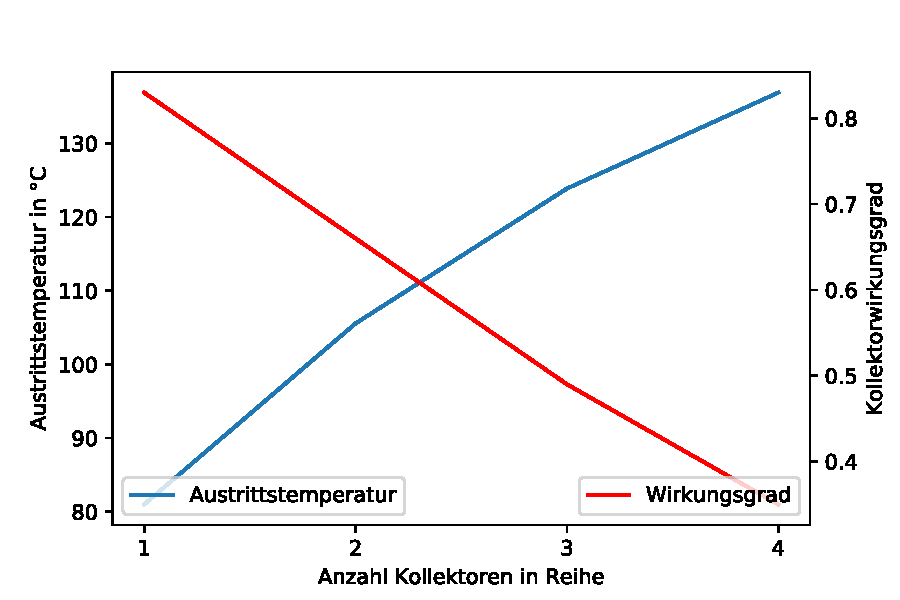
\includegraphics[width=0.8\linewidth]{Kollektortemperaturen.pdf}
		\captionof{figure}[Darstellung der Temperatur und des Wirkungsgrads einzelner Vakuumröhrenkollektoren mit zunehmender Kollektoranzahl]{Darstellung der Temperatur und des Wirkungsgrads einzelner Vakuumröhrenkollektoren mit zunehmender Kollektoranzahl bei gleichbleibendem Massenstrom. Während die Austrittstemperatur mit jedem zusätzlichen Kollektor zunimmt, sinkt der Wirkungsgrad des letzten Kollektors in Reihe.}
		\label{fig: Kollektortemperatur und Wirkungsgrad über Kollektoranzahl}
	\end{figure}
Abbildung \ref{fig: Kollektortemperatur und Wirkungsgrad über Kollektoranzahl} zeigt die entsprechende Abhängigkeit von der Austrittstemperatur. Der Verlauf des Wirkungsgrads impliziert, dass bei einer bestimmten Kollektoranzahl in Reihe der letzte Kollektor irgendwann - je nach Randbedingungen - einen negativen Wirkungsgrad aufweisen wird. Die Simulation in TESPy hat gezeigt, dass mehr Vakuumröhrenkollektoren als Flachkollektoren in Reihe geschaltet werden können, bevor der Wirkungsgrad negative Werte annimmt. Demgegenüber steht, dass Flachkollektoren derzeit die geringeren Investitionskosten aufweisen. Tabelle \ref{tab: verwendete Kollektordaten} gibt eine Übersicht über die wichtigsten Parameter bei der Simulation der Kollektoren. Das komplette \ac{TESPy}-Skript ist dem beigefügten Datenträger zu entnehmen.

Für die Optimierung eines solarthermisch gestützten Wärmesystems gilt es nun herauszufinden, welchen Einfluss eine Reihenschaltung auf den Wirkungsgrad des Gesamtsystems hat. Zu diesem Zweck sind für bis zu vier Kollektoren in Reihe die Systemwirkungsgrade über der Sonneneinstrahlung untersucht worden. Es zeigt sich, dass bei festgehaltener Austrittstemperatur eine Zunahme der Kollektoranzahl auf zwei, drei oder vier Kollektoren der Wirkungsgrad insgesamt relativ konstant bleibt. Bei geringer Einstrahlung ist eine leichte Abnahme des Wirkungsgrad mit zunehmender Kollektoranzahl zu beobachten. Bei einer höheren Einstrahlung von 600~W/m² bis 1000~W/m² ist praktisch kein Unterschied zu erkennen. Dieser Sachverhalt wird in Abbildung \ref{fig: TESPy Vergleich mehrerer Kollektoren in Reihe} dargestellt. Dieses Verhalten ist damit zu erklären, dass bei festgehaltener Reihen-Austrittstemperatur der Wirkungsgrad der hinteren Kollektoren sinkt, dem gegenüber jedoch eine Wirkungsgrad-Zunahme der vorderen Kollektoren, aufgrund der jeweils abnehmenden Kollektor-Austrittstemperatur, steht. 
	\begin{figure}[ht]
		\centering
		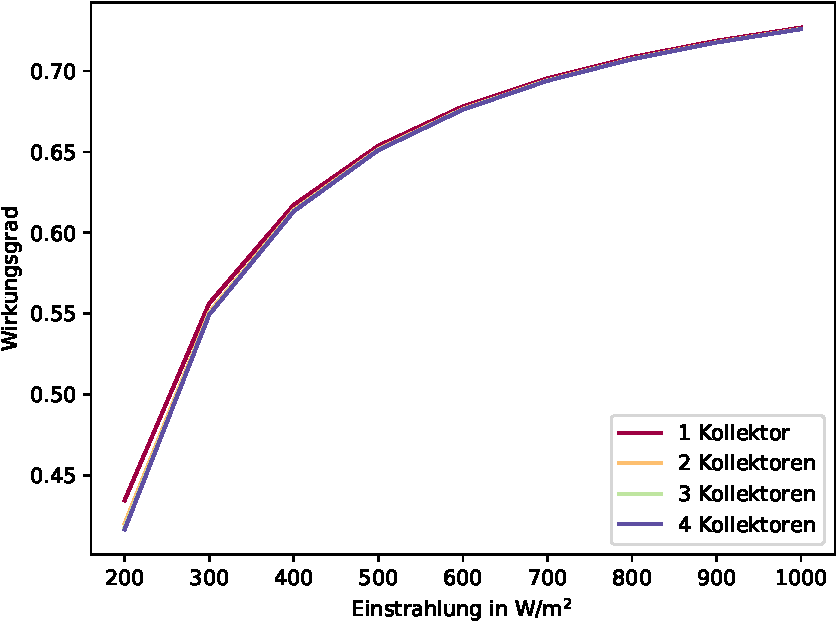
\includegraphics[width=0.8\linewidth]{Kollektor_eta_Reihe-cropped.pdf}
		\captionof{figure}[Vergleich des Gesamt-Wirkungsgrads mit zunehmender Kollektoranzahl in Reihe]{Darstellung des Gesamt-Wirkungsgrads mit zunehmender Kollektoranzahl in Reihe über einer variierenden Einstrahlung bei festgehaltener Austrittstemperatur anhand einer eigenen \ac{TESPy}-Simulation. Die Steigerung der Kollektoranzahl führt bei geringer Einstrahlung zu einer leichten Verringerung des Wirkungsgrads. Bei höherer Einstrahlung ist dieser Effekt nicht zu beobachten.}
		\label{fig: TESPy Vergleich mehrerer Kollektoren in Reihe}
	\end{figure}

Auf Grundlage der \ac{TESPy}-Simulation ist entschieden worden, die gewonnene Wärme des Kollektorfeldes über die DIN EN 12975 \cite{EN12975} für jeden Zeitschritt im Preprocessing zu berechnen und als Wert an Solph zu übergeben. Da der Unterschied zu einem einzelnen Kollektor quasi unerheblich ist, kann die DIN-Vorschrift bedenkenlos eingesetzt werden. Der Ertrag wurde folgendermaßen bestimmt:
	\begin{enumerate}
		\item Umrechnung der vorhandenen Einstrahlungsdaten auf die geneigte Ebene
		\item Nutzen der Vorlauf-, Umgebungstemperatur und Einstrahlungsdaten (vgl. Kapitel~\ref{section: Eingangsparameter der Optimierung}) zur Bestimmung des Kollektorwirkungsgrads nach DIN~EN~12975
		\item Berechnung des flächenspezifischen Ertrags der Solarthermie
	\end{enumerate} 

Auf Grund der Tatsache, dass der Wirkungsgrad eines Vakuumröhrenkollektors tendenziell höher ist, als der von Flachkollektoren ist entscheiden worden im weiteren Verlauf dieser Arbeit auf die Betrachtung von Flachkollektoren zu verzichten.

\section{Gas- und Dampfkraftwerk}\label{section: Gas- und Dampfkraftwerk}
Unter den verschiedenen Technologien der Kraft-Wärme-Kopplung ist das \acl{GuD} eine der bewährtesten Varianten. Die Abwärme der Gasturbine wird genutzt, um einen Dampfkreislauf zu betreiben und so die Brennstoffausnutzung weiter zu erhöhen. Im Vergleich zu Braun- oder Steinkohle gefeuerten Kraftwerken ist die CO$_2$-Emission von Gas gefeuerten Kraftwerken bezogen auf die Kilowattstunde Strom um mehr als die Hälfte geringer \cite{statista2019}. Der geplante Kohleausstieg der Bundesregierung für das Jahr 2038 erhöht die Bedeutung der \ac{GuD} weiter \cite{bmwi2019}. Aus diesem Grund wird in dieser Arbeit die \ac{GuD}-Technologie im Referenzsystem zur primären Wärmeversorgung verwendet.
	\begin{figure}[h]
		\centering
		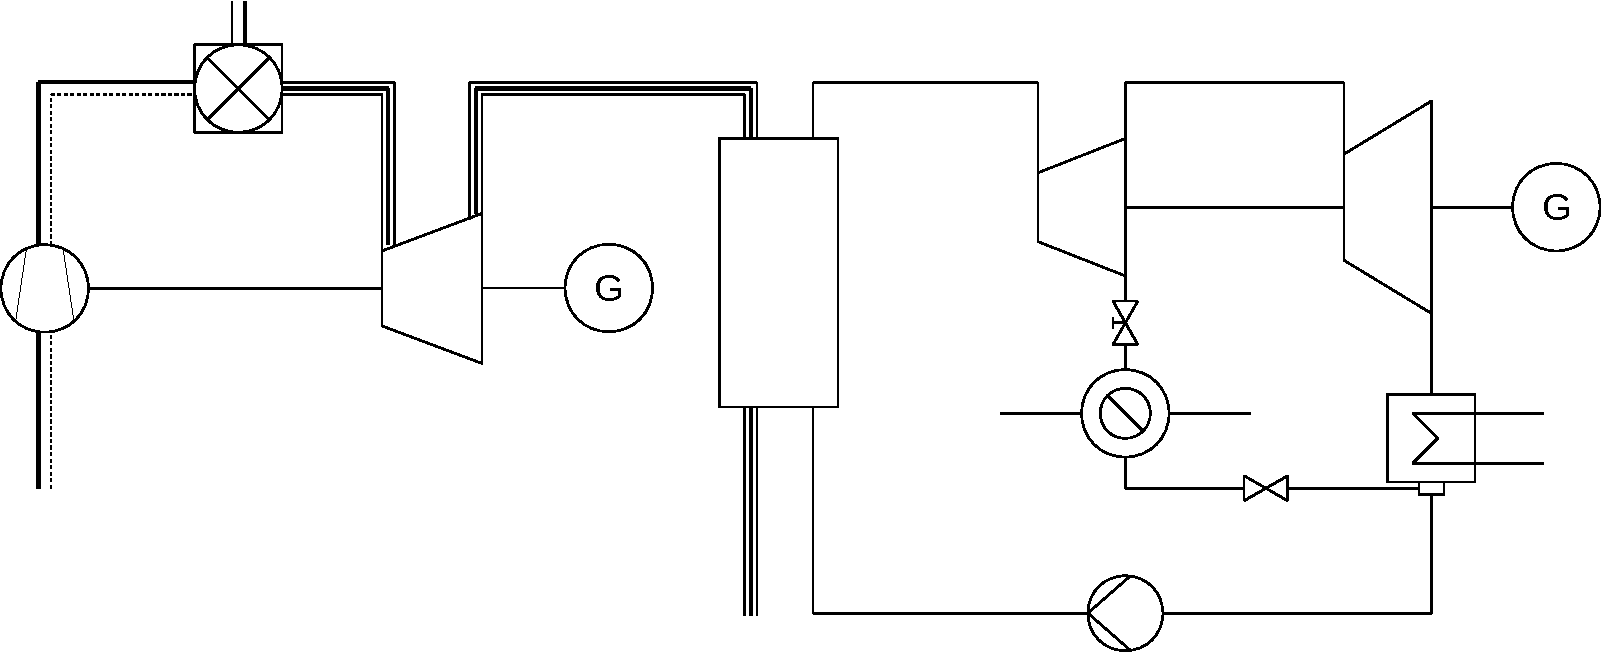
\includegraphics[width=0.8\linewidth]{SchaltplanGuD.pdf}
		\captionof{figure}{Wärmeschaltbild des in \ac{TESPy} modellierten \acl{GuD}s mit einer einfachen Entnahmeschaltung}
		\label{fig: Schaltplan GuD-Anlage}
	\end{figure}

Das verwendete Simulationsprogramm zur Optimierung des Energiesystems (Solph), auf das in Kapitel \ref{section: Solph} weiter eingegangen wird, verfügt bereits über eine \ac{GuD}-Komponente, die \textit{GenericCHP}, welche das Verhalten dieses Anlagentyps sehr genau beschreibt. Für eine detailliertere Beschreibung dieser Komponente wird entsprechend auf die \ac{oemof}-Dokumentation \cite{oemof2019} oder die Veröffentlichung von \citet{Mollenhauer2016} verwiesen, auf deren Grundlage die GenericCHP modelliert wurde. Um die GenericCHP-Komponente verwenden zu können sind nur einige Eckdaten nötig, die entsprechend über eine \ac{TESPy}-Simulation ermittelt worden sind. Die gewonnenen Eckdaten können in Tabelle \ref{tab: Notwendige Eckdaten zur Verwendung der GenericCHP-Komponente} nachgelesen werden.

Abbildung \ref{fig: Schaltplan GuD-Anlage} zeigt eine schematische Darstellung des modellierten Kraftwerks. Das nach der Expansion in der Gasturbine immer noch heiße Gas wird in einem Abhitzekessel genutzt, um Wärme für einen Dampfkraftprozess bereitzustellen. Der Dampfkreislauf ist als Entnahme-Kondensation ausgeführt, was bedeutet, dass Dampf der Turbine auf einem erhöhten Druckniveau zu Heizzwecken entnommen wird. Der Dampf wird in einem Heizkondensator kondensiert und gibt dabei Wärme an das Wärmenetz ab. Der in der Turbine verbleibende Dampf wird weiter auf einen niedrigeren Druck expandiert. Tabelle \ref{tab: Nennparameter GuD} fasst die wichtigsten Parameter zur Simulation des Kraftwerks zusammen.
	\begin{center}
		\captionof{table}{Notwendige Eckdaten zur Verwendung der GenericCHP-Komponente}
		\begin{tabular}{llll}
			\hline 
			\rule{0pt}{12pt} Parameter  & Symbol  & Einheit  & Wert \tabularnewline
			\hline 
			maximale elektrische Leistung ohne Wärmeauskopplung  & $P_\text{max,woDH}$ & MW & 406  \tabularnewline
			minimale elektrische Leistung ohne Wärmeauskopplung & $P_\text{min,woDH}$ & MW & 139 \tabularnewline
			maximale Stromausbeute ohne Wärmeauskopplung &  $\beta_\text{max,woDH}$  & - & 0,5851 \tabularnewline
			minimale Stromausbeute ohne Wärmeauskopplung &  $\beta_\text{min,woDH}$  & - & 0,4798 \tabularnewline
			Leistungs-Verlust-Index &  $beta$  & - & 0,2447 \tabularnewline
			\hline
			\label{tab: Notwendige Eckdaten zur Verwendung der GenericCHP-Komponente}  &  &  & 
		\end{tabular}
	\end{center} 

Diese Parameter werden von der GenericCHP-Komponente genutzt, um ein PQ-Diagramm der Anlage zu beschreiben. So kann jeder mögliche Betriebszustand der Anlage in der Optimierung abgebildet werden. Der Leistungs-Verlust-Index $beta$ gibt hierin das Maß der elektrischen Leistungsabnahmen, die mit einer zunehmenden Wärmeauskopplung einhergeht, an. 
\newpage
	\begin{center}
		\captionof{table}{Auslegungsparameter des Gas- und Dampfkraftwerks}
		%\renewcommand{\arraystretch}{1}
		\begin{tabular}{lllll}
			\hline 
			Teilprozess & Parameter  & Symbol  & Einheit  & Wert\tabularnewline
			\hline 
			\textbf{Fernwärme} & Vorlauftemperatur  & $T_{\text{VL}}$  & \textdegree C  &  124\tabularnewline
			& Rücklauftemperatur  & $T_{\text{RL}}$  & \textdegree C  & 50\tabularnewline
			& Druck  & $p_{\text{FW}}$  & bar  & 10\tabularnewline
			& Wärmeaufnahme & $\dot{Q}_\text{DH}$ & MW & 145 \tabularnewline
			\textbf{Gasturbinenprozess} & Brennstoffmassenstrom  & $\dot{m}_{\text{Fuel}}$  & kg/s  & 11,58 \tabularnewline
			& Umgebungstemperatur  & $T_{\text{U}}$  & \textdegree C & 20 \tabularnewline
			& Verbrennunstemperatur  & $T_{\text{CC}}$  & \textdegree C & 1500 \tabularnewline
			& Abgastemperatur  & $T_{\text{AG}}$  & \textdegree C & 150 \tabularnewline
			& Verdichterdruckverhältnis  & pr  & - & 14 \tabularnewline
			& Verdichterwirkungsgrad  & $\eta_{\text{V}}$  & - & 0,91 \tabularnewline
			& Gasturbinenwirkungsgrad  & $\eta_{\text{GT}}$  & - & 0,9 \tabularnewline
			\textbf{Dampfturbinenprozess} & Frischdampftemperatur  & $T_{\text{FD}}$  & \textdegree C & 600 \tabularnewline
			& Frischdampfdruck  & $p_{\text{FD}}$  & bar & 100 \tabularnewline
			& Entnahmedruck  & $p_{\text{E}}$  & bar & 3 \tabularnewline
			& Abdampfdruck  & $p_{\text{AD}}$  & bar & 0,04 \tabularnewline
			& Dampfturbinenwirkungsgrad  & $\eta_{\text{DT}}$  & - & 0,9 \tabularnewline
			& Pumpenwirkungsgrad  & $\eta_{\text{P}}$  & - & 0,8 \tabularnewline
			& Grädigkeiten  & $\Delta T$  & K & 5 \tabularnewline
			\hline 
			\label{tab: Nennparameter GuD}  &  &  & \tabularnewline
		\end{tabular}
	\par\end{center}
\newpage

\section{Kompressionswärmepumpe}\label{section: Modellbildung - Kompressionswärmepumpe}
	\begin{figure}
		\begin{subfigure}[b]{0.48\textwidth}
			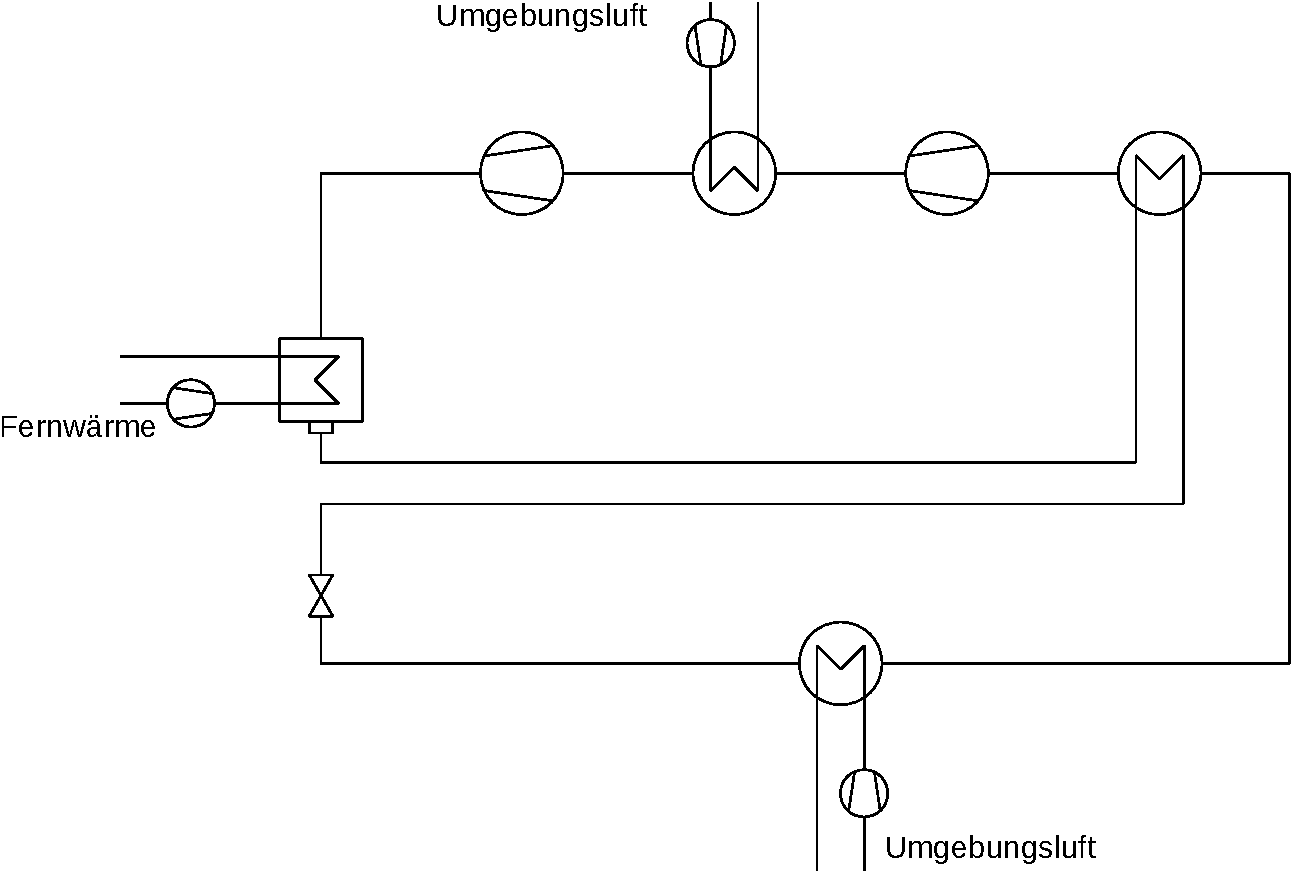
\includegraphics[width=1\textwidth]{Heatpump.pdf}
			\subcaption{Schaltbild}
			\label{subfigure: Schaltbild_Heatpump}
		\end{subfigure}
		\hfill
		\begin{subfigure}[b]{0.48\textwidth}
			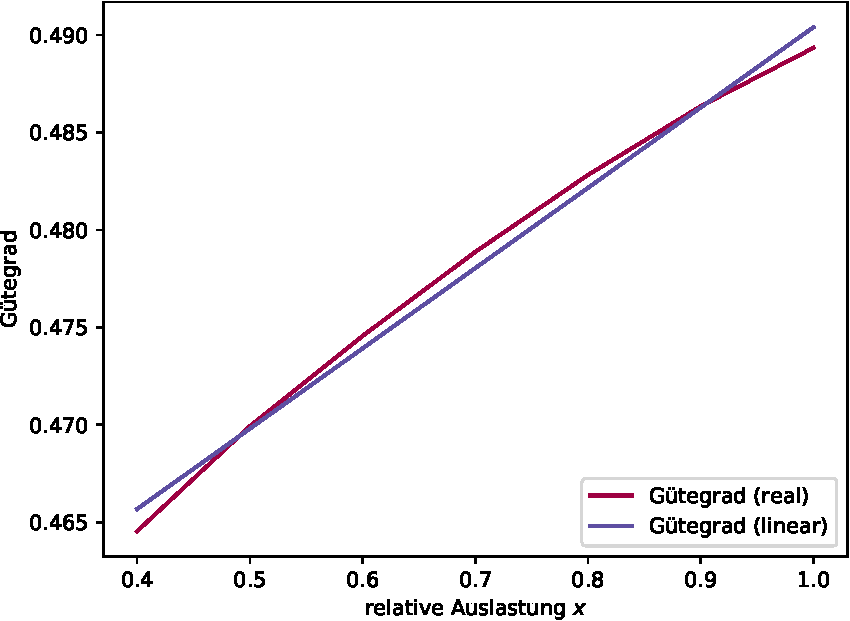
\includegraphics[width=1\textwidth]{Guetegrad_WP.pdf}
			\subcaption{}
			\label{subfigure: Guetegrad_WP}
		\end{subfigure}
		\caption[Konzeptionelle Darstellung zweier Ansätze zur Steigerung der Speicherkapazität durch Verwendung einer Wärmepumpe]{Schaltbild der modellierten Wärmepumpe (a) und Darstellung des Gütegrads über einer variierenden Auslastung (b)}
		\label{fig: HP - Schaltplan und Guetegrad}
	\end{figure}

Zur Bestimmung des Verhaltens der Wärmepumpe ist eine Ammoniak Kompressionswärmepumpe mit einfacher Unterkühlung in \ac{TESPy} abgebildet worden. Diese nutzt die Umgebungsluft als Wärmequelle. Ziel der Simulation ist die Bestimmung des Gütegrads über einem variierenden Lastbereich. Aus den vorliegenden Daten zur Umgebungstemperatur und der Vorlauftemperatur des Netzes sind Durchschnittswerte gebildet worden, für die die Wärmepumpe ausgelegt wurde. Diese Werte sind Tabelle \ref{tab: Randparameter der Wärmepumpe} zu entnehmen.
	\begin{center}
	\captionof{table}{Auslegungsparameter der Wärmepumpe}
	%\renewcommand{\arraystretch}{1}
	\begin{tabular}{lllll}
		\hline 
		Teilprozess & Parameter  & Symbol  & Einheit  & Wert\tabularnewline
		\hline 
		\textbf{Fernwärme} & Vorlauftemperatur  & $T_{\text{VL}}$  & \textdegree C  &  91,12\tabularnewline
		& Rücklauftemperatur  & $T_{\text{RL}}$  & \textdegree C  & 50\tabularnewline
		& Druck  & $p_{\text{FW}}$  & bar  & 10\tabularnewline
		& Wärmeaufnahme & $\dot{Q}_\text{DH}$ & MW & 145 \tabularnewline
		\textbf{Komponenten} & Verdichterwirkungsgrad  & $\eta_{\text{V,WP}}$  & - & 0,8 \tabularnewline
		& Verdichterdruckverhältnis  & $pr_\text{V}$  & - & 3,3 \tabularnewline
		& Druckverlust der Wärmeübertrager  & $pr_\text{WÜ}$  & - & 0,98 \tabularnewline
		& Lüfterwirkungsgrad  & $\eta_{\text{Lü}}$  & - & 0,6 \tabularnewline
		\textbf{Fluidwerte} & Sattdampfdruck  & $p_{\text{SD}}$  & bar & 6 \tabularnewline
		& Temperatur überhitzter Dampf & $T_{\text{ÜD}}$  & \textdegree C & 16 \tabularnewline
		& Eintrittstemperatur Verdichter 2  & $T_{\text{V2}}$  & \textdegree C & 60 \tabularnewline
		& abgegebener Wärmestrom  & $\dot{Q}_\text{WP}$  & MW & 25 \tabularnewline
		\hline 
		\label{tab: Randparameter der Wärmepumpe}  &  &  & \tabularnewline
	\end{tabular}
	\par\end{center}
Der Gütegrad der Wärmepumpe wird als Funktion der Verdichterleistung, aber nicht der Umgebungstemperatur oder Vorlauftemperatur des Netzes angenommen. Bei dieser Vereinfachung wird die Tatsache außer Acht gelassen, dass der Verdichter der Wärmepumpe mit zunehmender Vorlauftemperatur mehr arbeiten muss, um die gewünschte Temperatur überhaupt zu erreichen. Dieser Fehler wird für eine einfachere Beschreibung jedoch akzeptiert. Die gewonnene Kennlinie kann Gleichung \ref{equation: KennlinieHP} entnommen werden, welche den Gütegrad in Abhängigkeit der relativen Auslastung $x$ der Wärmepumpe darstellt. Der Gütegrad wird zusammen mit einem Schaltbild der modellierten Wärmepumpe in Abbildung \ref{fig: HP - Schaltplan und Guetegrad} dargestellt. 
	\begin{equation}\label{equation: KennlinieHP}
		\eta_\text{WP} = \text{0,0412} x + \text{0,4492}
	\end{equation}

Gleichung \ref{equation: Leistungszahl 1} zeigt, wie die Leistungszahl der Wärmepumpe von der Carnot-Leistungszahl und dem Gütegrad abhängt. Zur Verwendung in Solph ist die Carnot-Leistungszahl im preprocessing für jeden Zeitschritt anhand der Umgebungstemperatur und Vorlauftemperatur berechnet worden und wird als Liste an Solph übergeben. Abbildung \ref{fig: Kennfeld_HP} zeigt die möglichen Leistungszahlen während der Optimierung. Je nach Last und Vorlauf- bzw. Umgebungstemperatur kann in dem Diagramm die aus dem Gütegrad und der Carnot-Leistungszahl resultierende Leistungszahl der Wärmepumpe abgelesen werden.

Zur Implementierung in Solph ist die Komponente \textit{OffSetTransformer} verwendet worden, um zu gewährleisten, dass eine minimale Verdichterleistung bei der Optimierung nicht unterschritten werden kann. Das vollständige Modell und alle Randparameter können dem beigefügten Datenträger entnommen werden.

	\begin{figure}[ht]
		\centering
		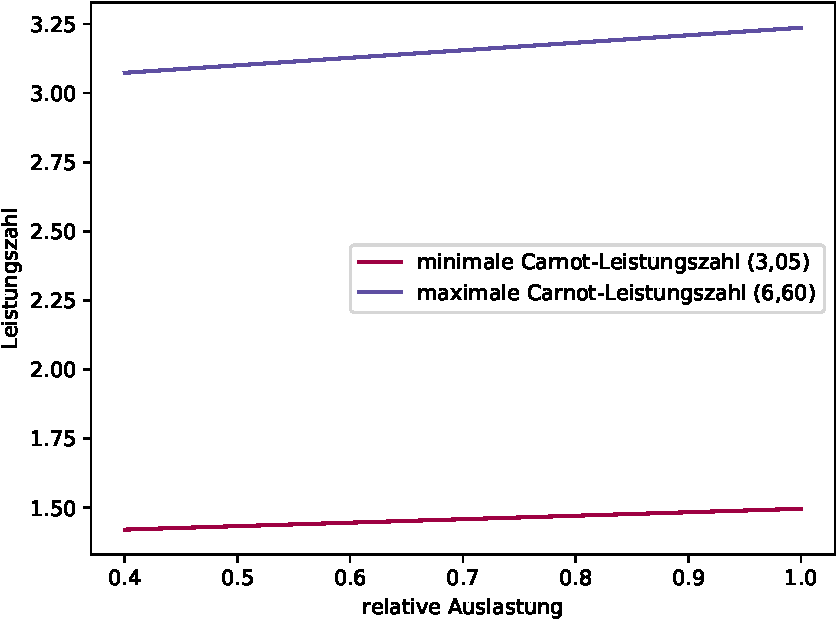
\includegraphics[width=0.8\linewidth]{Kennfeld_HP-cropped.pdf}
		\captionof{figure}[Kennfeld der modellierten Wärmepumpe]{Kennfeld der modellierten Wärmepumpe. Die untere Linie stellt, je nach Auslastung, die minimal mögliche Leistungszahl dar ($\varepsilon_\text{WPC,min}=3,05$) - entsprechend stellt die obere Linie die maximal erreichbare Leistungszahl dar ($\varepsilon_\text{WPC,max}=6,60$). Während der Optimierung operiert die Wärmepumpe stets innerhalb dieser Grenzen.}
		\label{fig: Kennfeld_HP}
	\end{figure}

\section[Sonstige Technologien]{Sonstige Technologien - Wärmespeicher, Elektrodenheizkessel, Spitzenlastkessel und Photovoltaik}
Für Wärmespeicher, Elektrodenheizkessel, Spitzenlastkessel und die \ac{PV}-Anlage sind keine eigenen Simulationen zum Betriebsverhalten durchgeführt worden. Bei jeder dieser Komponenten ist für die Optimierung von einem konstanten Wirkungsgrad ausgegangen worden. Der Wirkungsgrad des Spitzenlastkessel ist über das in Abbildung \ref{fig: Volta-Feuerung} dargestellte Diagramm zur Bestimmung des feuerungstechnischen Wirkungsgrades \cite{Volta2018} abgeschätzt worden. Dargestellt wird der Wirkungsgrad bei variierendem Verbrennungsluftverhältnis über der Rauchgastemperatur. Bei der Abschätzung des Wirkungsgrades ist von einem Verbrennungsluftverhältnis $\lambda = 1$ und gerade keiner Kondensation im Rauchgas (Taupunkt) ausgegangen worden. Der Wirkungsgrad des \acl{EHK} ist einem Übersichtsblatt für verschiedene Erzeugungsanlagen der \textit{Danish Energy Agencey} \cite{Energinet} entnommen.
	\begin{figure}[ht]
		\centering
		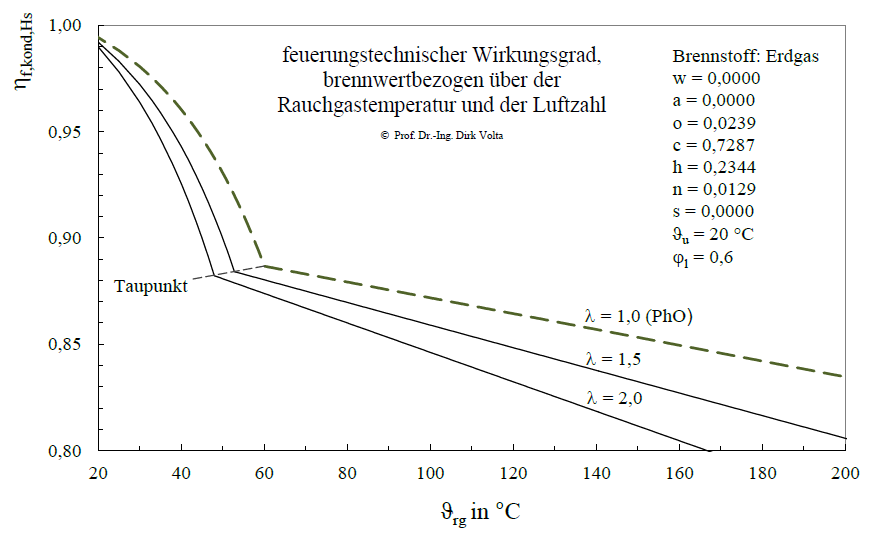
\includegraphics[width=0.8\linewidth]{Volta-Feuerung.png}
		\captionof{figure}[Darstellung des feuerungstechnischen Wirkungsgrads über der Rauchgastemperatur]{Darstellung der Abhängigkeit des feuerungstechnischen Wirkungsgrads über der Rauchgastemperatur für unterschiedliche Verbrennungsluftverhältnisse übernommen aus \cite{Volta2018}}
		\label{fig: Volta-Feuerung}
	\end{figure}

Für die \acl{PV} ist, wie bei der Solarthermie auch, der Anlagen-Ertrag im Preprocessing über Gleichung \ref{equation: LeistungPV} berechnet worden. Der Wirkungsgrad der Module wurde hierbei dem \textit{Photovoltaics Report} \cite{ISE10}, der die durchschnittliche Effizienz von Silizium basierten Modulen mit 17\% angibt, entnommen. Der Wirkungsgrad des Wechselrichters und ein Wert für den Performance Ratio in Deutschland konnten hingegen über \textit{Aktuelle Fakten zur Photovoltaik in Deutschland} \cite{ISE} identifiziert werden. 

Die Wärmespeicher sind als sensible Wärmespeicher angenommen worden. Der entsprechende Wirkungsgrad ist \citet{Kaldemeyer2019} zu entnehmen. In Tabelle \ref{tabelle: Wirkungsgrade Speicher, EHK, SLK und PV} werden alle angenommenen Wirkungsgrade für den Speicher, \acl{EHK}, \acl{SLK} und die \ac{PV}-Anlage aufgelistet. 

	\begin{center}
	\captionof{table}{Wirkungsgrade für Wärmespeicher, Elektrodenheizkessel, Spitzenlastkessel und Photovoltaik}
	\label{tabelle: Wirkungsgrade Speicher, EHK, SLK und PV}
		\begin{tabular}{llclc}
			\hline 
			\rule{0pt}{12pt} Komponente  & Symbol  & Einheit  & Wert & Quelle\tabularnewline
			\hline 
			Wärmespeicher  & $\eta_\text{sp}$  & - & 0,75 & \cite{Kaldemeyer2019}  \tabularnewline
			Elektrodenheizkessel  & $\eta_\text{ehk}$ & - & 0,99 &\cite{Energinet} \tabularnewline
			Spitzenlastkessel  & $\eta_\text{slk}$ & - & 0,88 &\cite{Volta2018} \tabularnewline
			\textbf{Photovoltaik} & & & &\tabularnewline
			Modul  & $\eta_\text{pv}$  & - & 0,17 &\cite{ISE10}  \tabularnewline
			Wechselrichter  & $\eta_\text{wr}$  & - & 0,98 &\cite{ISE}  \tabularnewline
			Performance Ratio  & PR  & - & 0,85 &\cite{ISE}  \tabularnewline
			\hline
		\end{tabular}
	\end{center} 
